\chapter{Resultados}

Este trabalho tem como objetivo realizar o controle da posição linear de um carro. Com o sistema de controle agora elaborado, este foi colocado a teste tanto em um ambiente de simulação quanto na bancada, neste capítulo são apresentados os resultados obtidos.

\section{Resultados de simulação}

As simulações foram conduzidas em Python, empregando o modelo matemático descrito no Capítulo 2 e o sistema de controle desenvolvido no Capítulo 3.

Com o objetivo de tornar o comportamento simulado mais representativo do sistema real, foram incorporados ao modelo uma zona morta de 3 V e uma saturação do canal de entrada limitada a ± 12 V. Esses efeitos não lineares refletem características físicas observadas experimentalmente. 

Para a avaliação do desempenho do controlador, foi adotada uma referência do tipo degrau, aplicada após 1 s de simulação. As Figuras \ref{fig:simulacao01m} e \ref{fig:simulacao02m} apresentam a resposta para para degraus de referência, respectivamente, de 0,1 m e 0,2 m. Em ambas as figuras, é possível observar que o carro convergiu para a posição de referência. Ademais, constata-se a ocorrência de saturação no canal de entrada, embora de forma transitória e de curta duração.

\begin{figure}[H]
    \centering
    \includegraphics[width=0.8\linewidth]{figuras/simulacao_referencia_01m.eps}
    \caption[Simulação do comportamento do sistema em malha fechada considerando a referência de amplitude $0,1$~m. Na figura superior, tem-se a evolução temporal da posição do carro, e na segunda da tensão aplicada ao motor]{Simulação do comportamento do sistema em malha fechada considerando a referência de amplitude $0,1$~m. Na figura superior, tem-se a evolução temporal da posição do carro, e na segunda da tensão aplicada ao motor.}
    \label{fig:simulacao01m}
\end{figure}

\begin{figure}[H]
    \centering
    \includegraphics[width=0.8\linewidth]{figuras/simulacao_referencia_02m.eps}
    \caption[Simulação do comportamento do sistema em malha fechada considerando a referência de amplitude $0,2$~m]{Simulação do comportamento do sistema em malha fechada considerando a referência de amplitude $0,2$~m.}
    \label{fig:simulacao02m}
\end{figure}

É importante destacar que a presença dos efeitos não lineares na simulação faz com que os requisitos de projeto não sejam atendidos com exatidão nas simulações. Entretanto, o fato de que o carro é guiado para próximo da referência indica que o sistema de controle funcionará corretamente na prática, a despeito de tais efeitos. Isso será avaliado na sequência.

\section{Resultados experimentais}

O mesmo tipo de entrada foi aplicada nos testes experimentais, uma referência do tipo degrau. As Figuras \ref{fig:controlador01m} e \ref{fig:controlador02m} apresentam as respostas obtidas para amplitudes de degrau de, respectivamente, $0,1$~m e $0,2$~m. Observa-se que em todos os casos, a entrada da planta satura no início, ou seja, no momento que é necessário vencer o atrito seco e colocar o carro em movimento, após isso a entrada da planta não satura mais. 

Pode-se afirmar que, na prática, a resposta observada se assemelha a de um sistema de primeira ordem. Mesmo assim, considera-se que o sistema de controle atingiu o principal objetivo proposto: Guiar o carro para a referência de posição.


\begin{figure}[H]
    \centering
    \includegraphics[width=0.8\linewidth]{figuras/controlador_referencia_01m.eps}
    \caption[Dados experimentais do controlador com referência de $0,1$~m]{Dados experimentais do controlador com referência de $0,1$~m.}
    \label{fig:controlador01m}
\end{figure}

\begin{figure}[H]
    \centering
    \includegraphics[width=0.8\linewidth]{figuras/controlador_referencia_02m.eps}
    \caption[Dados experimentais do controlador com referência de $0,2$~m]{Dados experimentais do controlador com referência de $0,2$~m.}
    \label{fig:controlador02m}
\end{figure}

Pode ser observado que as limitações físicas da planta tornam o sistema mais lento, fazendo com que o carro para de se movimentar no momento que atinge a sua posição de referência, mesmo que no instante que atinja ainda exista ação de controle. Assim, não existe erro de regime estacionário, mesmo que não ocorra nem máximo sobressinal e nem tempo de pico. 

\section{Comparação entre os Resultados}

Com os resultados obtidos tanto em simulacão quanto os experimentais, foram plotadas as respostas para uma entrada degrau de referência de $0,2$~m  Os resultados podem ser observados na Figura \ref{fig:controlador_comparacao}.

\begin{figure}[H]
    \centering
    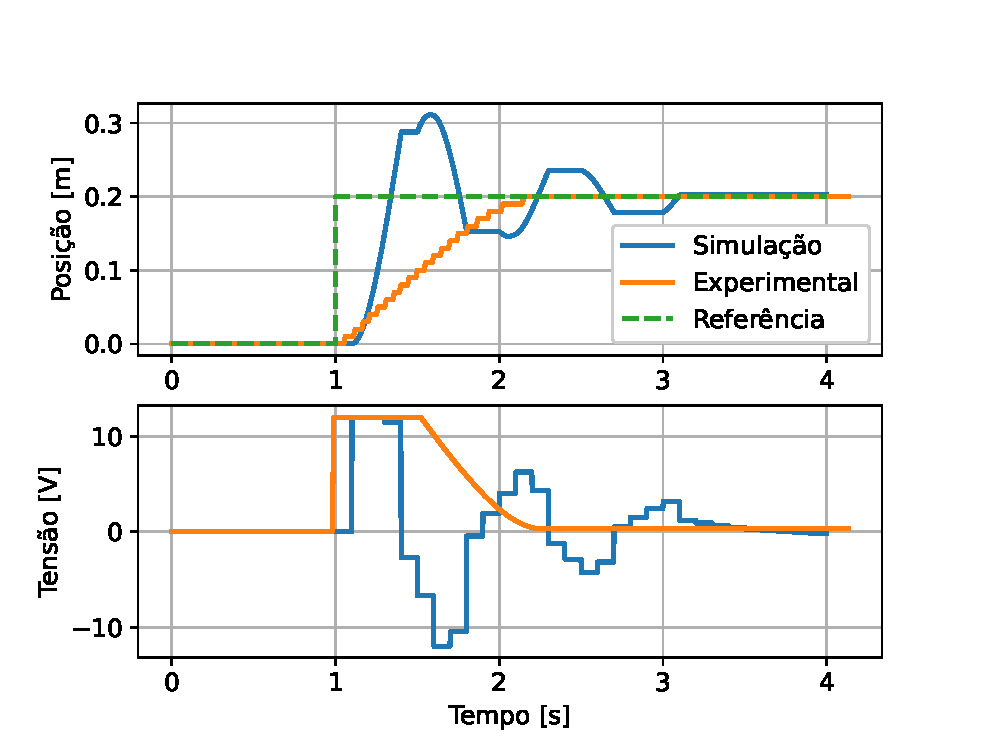
\includegraphics[width=0.8\linewidth]{figuras/controlador_comparacao.eps}
    \caption[Comparação entre os dados experimentais e simulação do controlador com referência de $0,2$~m]{Comparação entre os dados experimentais e simulação do controlador com referência de $0,2$~m.}
    \label{fig:controlador_comparacao}
\end{figure}

Em ambos os casos as limitações da planta provocam uma diferença com os requisitos de projeto estipulados, entre elas a mais significante é a zona morta do motor. Mesmo assim, tanta na simulação quanto no experimento o carro atinge a posição desejada e elimina o erro de regime estacionário, embora tenha respostas distintas no regime transiente. A discrepância observada entre os resultados experimentais e os obtidos por simulação pode ser atribuída à natureza não linear do atrito, a pequenas imperfeições na construção da bancada experimental e a incertezas nos parâmetros do modelo, como a constante de torque, a resistência da armadura e o ganho do atuador. Tais fatores afetam diretamente a precisão da modelagem e, consequentemente, a concordância entre os resultados simulados e experimentais.